\documentclass{beamer}
\usetheme{CambridgeUS}
\useinnertheme{rectangles}

\usepackage{amssymb, amsmath}
\usepackage[utf8]{inputenc}
\usepackage{babel}
\usepackage[T1]{fontenc}
\usepackage[autostyle=true]{csquotes}
\usepackage{hyperref}

\newcommand{\red}[1]{\textcolor{red}{#1}}
\newcommand{\blue}[1]{\textcolor{blue}{#1}}

\setbeamertemplate{caption}{\raggedright\insertcaption\par} 
\setbeamertemplate{bibliography item}{\insertbiblabel}

\newcommand{\backupbegin}{
   \newcounter{framenumberappendix}
   \setcounter{framenumberappendix}{\value{framenumber}}
}
\newcommand{\backupend}{
   \addtocounter{framenumberappendix}{-\value{framenumber}}
   \addtocounter{framenumber}{\value{framenumberappendix}} 
}

\title[Corner Region Inpainting]{Exploring Circular Corner Regions as Seed Points for PDE-based Inpainting}
\author{Daniel Gusenburger}

\begin{document}

\begin{frame}[t]
        \titlepage
\end{frame}


%~~~~~~~~~~~~~~~~~~~~~~~~~~~~~~~~~~~~Introduction~~~~~~~~~~~~~~~~~~~~~~~~~~~~~~~~~~~~~~~~~
    \section{Motivation}
    \begin{frame}[t]
        \frametitle{What is inpainting\dots}
        \begin{figure}
            \centering
            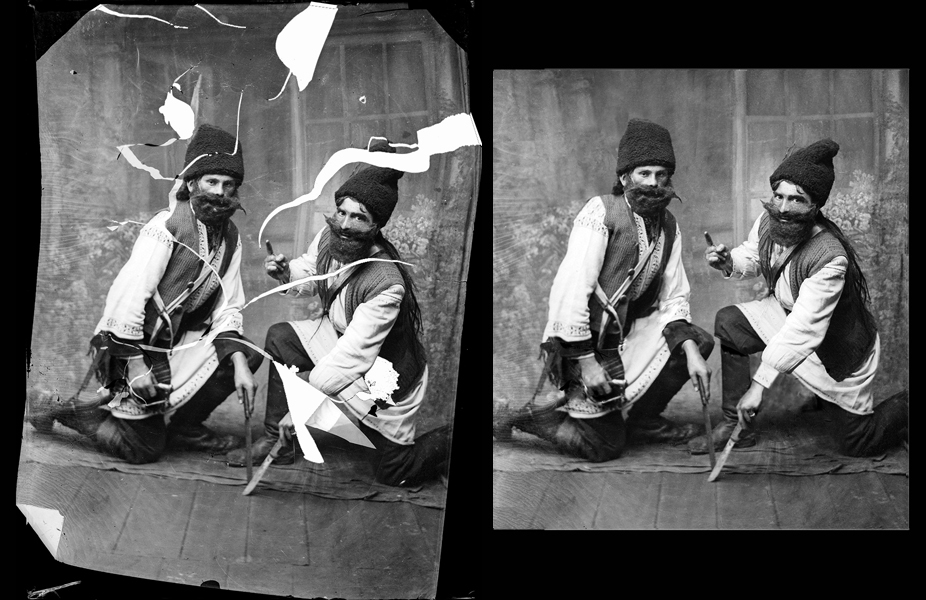
\includegraphics[width=0.5\linewidth]{../thesis/Images/Digital_Image_Restoration_and_Reconstraction.jpg}
            \caption{\tiny{\url{https://upload.wikimedia.org/wikipedia/commons/a/ae/Digital_Image_Restoration_and_Reconstraction.jpg}}}
        \end{figure}
        \vspace{-1em}
        \begin{itemize}
            \item Restoration technique (antique paintings etc.)
            \item Used for decades
            \item Digital inpainting introduced in 2000
        \end{itemize}
    \end{frame}

    \begin{frame}[t]
        \frametitle{\dots and why do we care?}
        \begin{block}{Image Compression}
            Inpainting based image compression methods are already able to outperform traditional
            codecs like JPEG for high compression rates 
        \end{block}
        \visible<2->
        {
            \begin{figure}
                \centering
                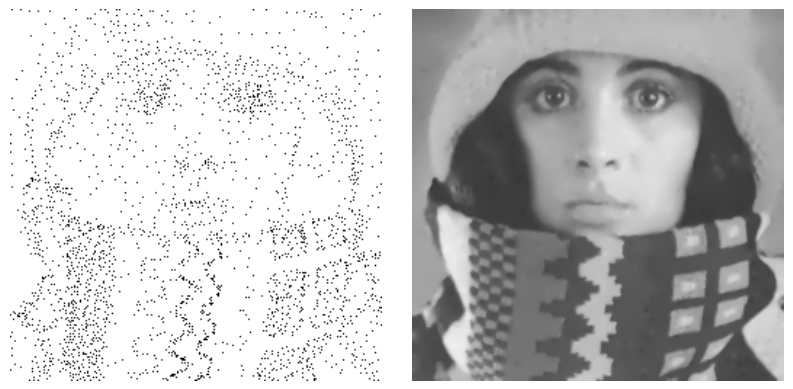
\includegraphics[width=0.6\linewidth]{../thesis/Images/pde_example.png}
                \caption{Source:~\cite{hoeltgen15}}
            \end{figure}
        }
    \end{frame}

    \begin{frame}[t]
        \frametitle{Problem description}
        \begin{itemize}
            \item<+-> Choosing optimal seed points for PDE-based inpainting is not trivial
            \item<+-> Many different approaches (semantic, tree-based, analytic, \dots)
            \item<+-> \red{Semantic:} use image features as seeds (edges/corners)
            \item<+-> Edge-based methods successful
            \item<+-> Corners as seed points barely explored
        \end{itemize}
    \end{frame}

    \section{Related Work}
    \begin{frame}[t]
        \frametitle{Related Work}
        \textit{PDE-based inpainting using corner information (Zimmer, 2007)}
        \visible<1-3,5-> {
            \begin{itemize}
                \item<+-> Examined how well images can be compressed using only corners
                \item<+-> Masks as small neighbourhood around important corners
                \item<+-> Reconstruction using mean curvature motion (MCM) + edge-enhancing diffusion
                    (EED) 
                \item<+-> Open potential:
                    \begin{itemize}
                        \item Corner detection very fuzzy (example results) 
                        \item Corner regions not optimised properly
                        \item MCM not well suited for inpainting
                    \end{itemize}
            \end{itemize}     
        }
        \only<4> {
            \vspace{-4cm}
            \begin{figure}
                \centering
                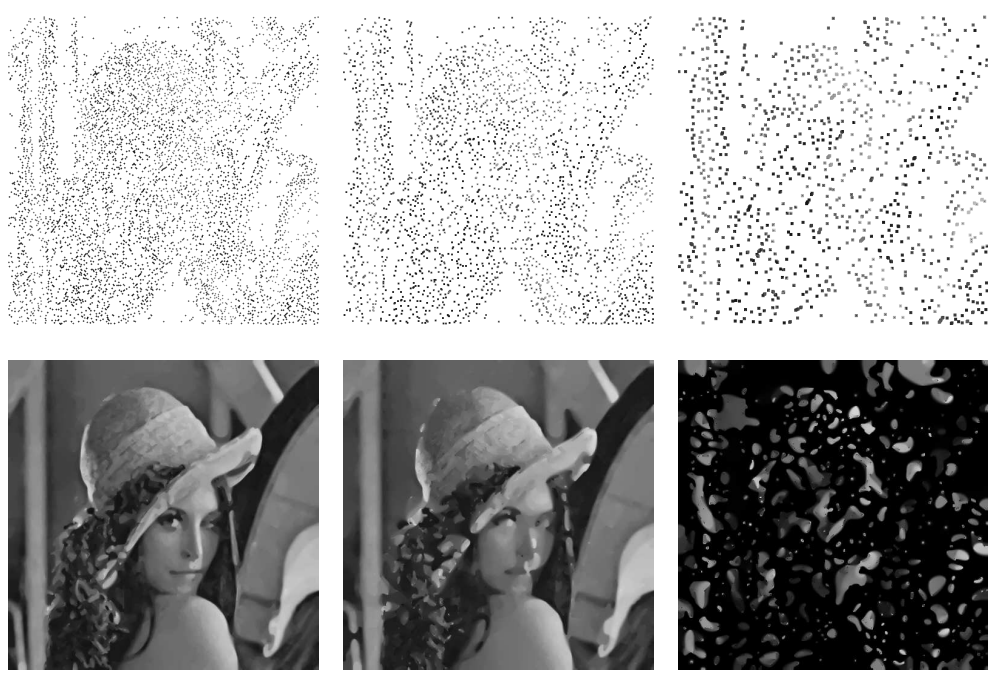
\includegraphics[width=0.7\linewidth]{../thesis/Images/zimmer_result.png}
                \caption{Inpainting results from~\cite{zimmer07} for corner regions of different sizes}
         \end{figure}
        }
    \end{frame}

    \section{Approach}
    \subsection{Overview}
    \begin{frame}[t]
        \frametitle{Approach}
        \begin{block}{Idea}<+->
            What if instead of only a small neighbourhood around each corner, we kept a large disc?  
        \end{block}
        \begin{block}{Approach}<+->
            \begin{itemize}
                \item Follow up on approach of Zimmer
                \item Förstner-Harris corner detection 
                \item Introduce modifications
                    \begin{itemize}
                        \item to better control mask size
                        \item to adapt detection to circular corner regions
                    \end{itemize}
                \item Pure EED inpainting
                \item Quantitative evaluation using \textbf{MSE}/\textbf{PSNR}
            \end{itemize}
        \end{block}
    \end{frame}

    \begin{frame}[t]
        \frametitle{Structure tensor based corner detection}
        \visible<1-3,5->{
            \begin{itemize}
                \item<+-> Structure tensor averages directional information in the
                    surrounding region
                    \[ J_\rho = K_\rho * (\nabla u\nabla u^\top) \]
                \item<+-> Corner detection based on eigenvalues 
                \item<+-> Förstner-Harris measure:
                    \[ \det(J) / \text{tr}(J) = \frac{\lambda_1\lambda_2}{\lambda_1 + \lambda_2} > T\]
                \item<5-> Local maxima of this measure are marked as corners
            \end{itemize} 
        }
        \only<4> {
            \vspace{-5cm}
            \begin{figure}
                \centering
                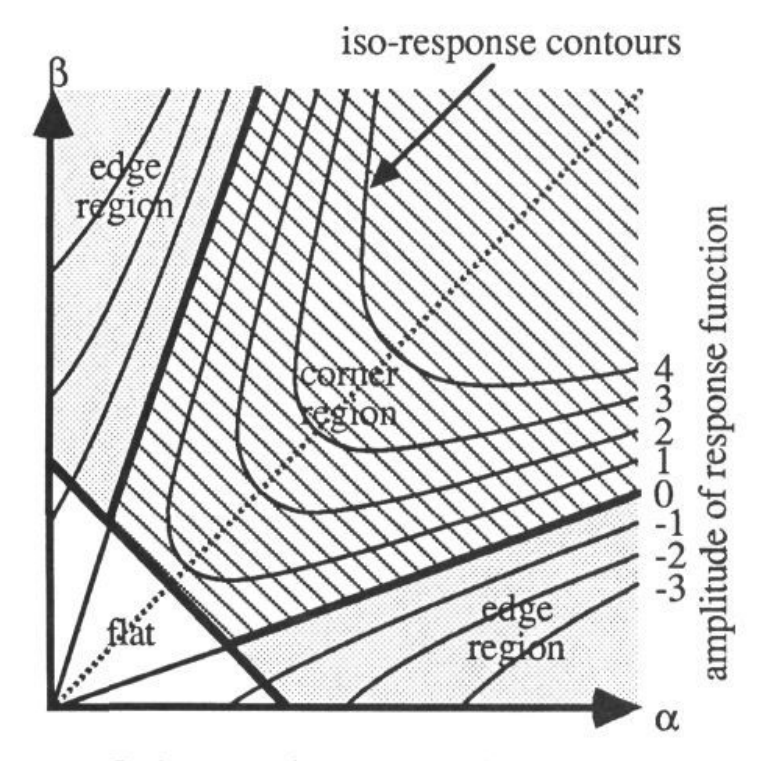
\includegraphics[height=0.6\textheight]{../thesis/Images/structure_tensor.png}
                \caption{Visualization of relation between eigenvalues of structure tensor. Source:
\cite{harris88}}
            \end{figure}
        }
    \end{frame}


    \subsection{Modifications}
    \begin{frame}[t]
        \frametitle{Percentile Thresholding}
        \begin{block}{Problem}<+->
            Amount of corners varying on input image with fixed threshold\\
            Makes it hard to reliably produce masks of the same size
        \end{block}
        \begin{block}{Remedy}<+->
            Use so called percentile on cornerness map to filter out a certain percentage of
            corners
        \end{block}
        \begin{block}{Alternative}<+->
            Instead of filtering out percentage of corners, calculate upper bound for number of
            corners such that only a certain percentage of \textit{pixels} is kept.
        \end{block}
    \end{frame}  
     \begin{frame}[t]
        \frametitle{Non-maximum Suppression}
        \begin{block}{Observation}
            Corner regions tend to overlap a lot, especially in textured regions\\
            Results in poorly distributed inpainting mask
        \end{block} 
        \begin{block}{Possible Remedy}
            Discard corners already covered by a `better' corner 
        \end{block}
     \end{frame} 

    \begin{frame}[t]
        \frametitle{Non-maximum suppression}
        \begin{figure}
            \centering
            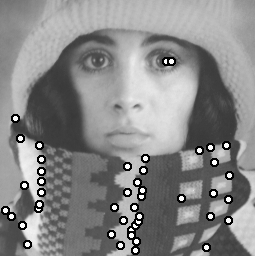
\includegraphics[width=0.4\linewidth]{../thesis/Images/trui_corners_non_cnms.png}
            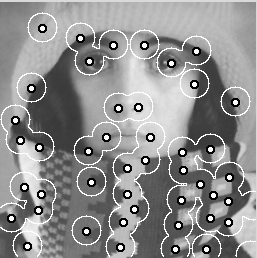
\includegraphics[width=0.4\linewidth]{../thesis/Images/trui_corners_cnms_influence.png}
            \caption{\textbf{Left:} Centre points of corner regions without suppression. \textbf{Right:} With
            suppression (boundary of each region highlighted). Corner detection using
        Förstner-Harris detector with identical parameters}
        \end{figure}
    \end{frame}

    \begin{frame}[t]
        \frametitle{Expectations and Limitations}
        \begin{figure}
             \centering
             
\includegraphics[width=0.3\linewidth]{../images/binary/abstract1.png}
             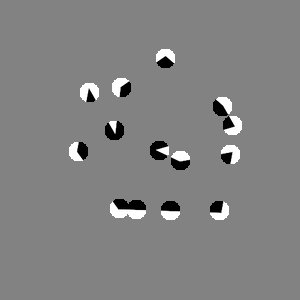
\includegraphics[width=0.3\linewidth]{../thesis/Images/abstract1_small-mask.png}
             
\includegraphics[width=0.3\linewidth]{../thesis/Images/abstract_small_inpaint.png}
             \caption{\textbf{Left:} Mask ($\approx5\%$ of all pixels). \textbf{Right:} Inpainting result
             ($\sigma=4,\lambda=0.03$, stopped after 1000 iterations with $\tau=1000$) PSNR=32.04}
         \end{figure} 
    \end{frame}

    \begin{frame}
        \frametitle{Expectations and Limitations}
        \begin{figure}
             \centering
             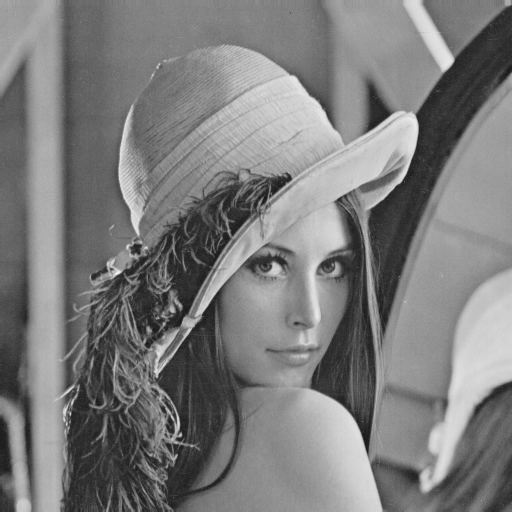
\includegraphics[width=0.3\linewidth]{../images/grey/lena512.png}
             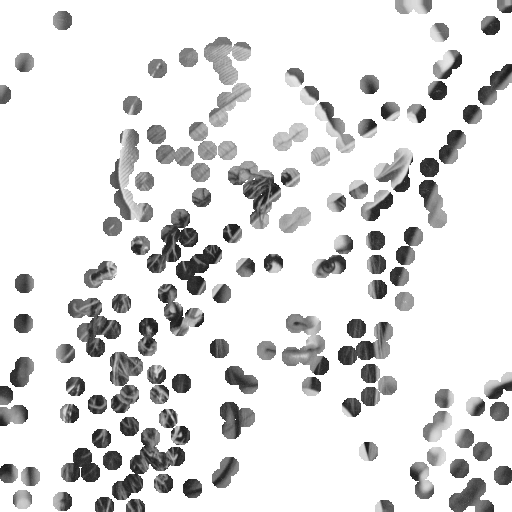
\includegraphics[width=0.3\linewidth]{../thesis/Images/lena512-mask.png}
             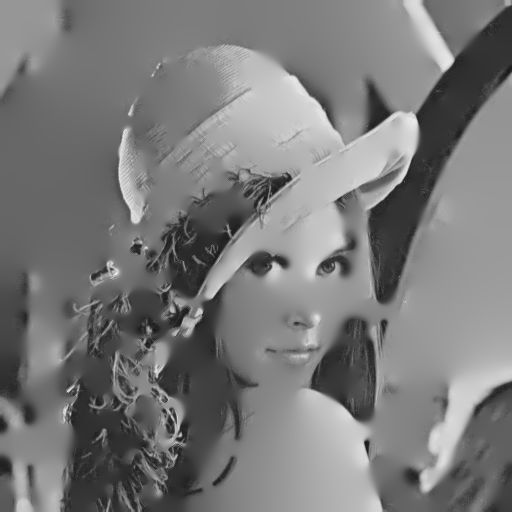
\includegraphics[width=0.3\linewidth]{../thesis/Images/lena512-inpaint.png}
             \caption{\textbf{Left:} Original image \textit{lena512}. \textbf{Middle:} Mask (filled
                 with white for visualisation, $\approx20\%$ of all pixels) \textbf{Right:} Inpainting result
             ($\sigma=2,\lambda=0.4$, stopped after 1000 iterations with $\tau=1000$) PSNR=21.56}
        \end{figure}    
    \end{frame}

    %\begin{frame}[t]
        %\frametitle{Limitations}
        %\begin{block}{What the approach may struggle with\dots}<+->
            %\begin{itemize}
                %\item Images with very few corners (e.g.\ barcodes/parallel lines?)
                %\item Highly textured images 
                %\item Noisy images
            %\end{itemize}   
        %\end{block}
        %\begin{block}{Where I expect it to do well\dots}<+->
            %\begin{itemize}
                %\item Comic-style images
                %\item Binary images
            %\end{itemize}
         %\end{block} 
    %\end{frame}

    \begin{frame}
        \centering\huge{Any questions?}
    \end{frame}

    \begin{frame}
        \centering\huge{Thank you for your time!}
    \end{frame}

%~~~~~~~~~~~~~~~~~~~~~~~~~~~~~~~~~~~~References~~~~~~~~~~~~~~~~~~~~~~~~~~~~~~~~~~~~~~~~~~~
    \section{References}
    \begin{frame}[t]
        \frametitle{Bibliography}
        \bibliographystyle{apalike}
        \bibliography{../thesis/references.bib}
    \end{frame}

    \backupbegin
    \section*{Appendix}

    \begin{frame}
        \frametitle{Examples (3)}
        \begin{figure}
             \centering
             
\includegraphics[width=0.3\linewidth]{../images/binary/abstract1_noise.png}
             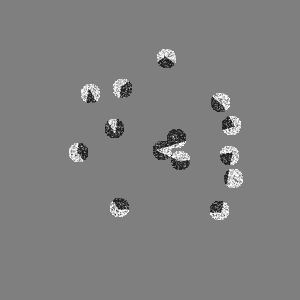
\includegraphics[width=0.3\linewidth]{../thesis/Images/abstract1_noise_mask.png}
             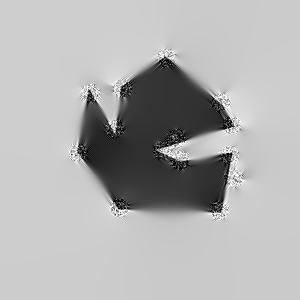
\includegraphics[width=0.3\linewidth]{../thesis/Images/abstract1_noise_inpaint.png}
             \caption{\textbf{Left:} Original image. \textbf{Middle:} Mask ($\approx5\%$ of all
                 pixels) \textbf{Right:} Inpainting result
             ($\sigma=4,\lambda=0.3$, stopped after 1000 iterations with $\tau=1000$) PSNR=16.72}
        \end{figure}    
    \end{frame}
    \backupend

\end{document}
